\section{AND}

\subsection{Checking if a value is on $2^n$ boundary}

If you need to check if your value is divisible by $2^n$ number (like 1024, 4096, etc.) without remainder,
you can use a \TT{\%} operator in \CCpp, but there is a simpler way.
4096 is 0x1000, so it always has $4*3=12$ lower bits cleared.

What you need is just:

\begin{lstlisting}[style=customc]
if (value&0xFFF)
{
	printf ("value is not divisible by 0x1000 (or 4096)\n");
	printf ("by the way, remainder is %d\n", value&0xFFF);
}
else
	printf ("value is divisible by 0x1000 (or 4096)\n");
\end{lstlisting}

In other words, this code checks if there are any bit set among lower 12 bits.
As a side effect, lower 12 bits is always a remainder from division a value by 4096 (because division by $2^n$
is merely a right shift, and shifted (and dropped) bits are bits of remainder).

Same story if you want to check if the number is odd or even:

\begin{lstlisting}[style=customc]
if (value&1)
	// odd
else
	// even
\end{lstlisting}

This is merely the same as if to divide by 2 and get 1-bit remainder.

\subsection{KOI-8R Cyrillic encoding}

It was a time when 8-bit \ac{ASCII} table wasn't supported by some Internet services, including email.
Some supported, some others---not.

It was also a time, when non-Latin writing systems used second half of 8-bit ASCII table to accommodate non-Latin characters.
There was several popular Cyrillic encodings, but KOI-8R (devised by Andrey ``ache'' Chernov)
is somewhat unique in comparison with others.

% TODO invert arrow 
% TODO text latex form instead of png!
\begin{figure}[H]
\centering
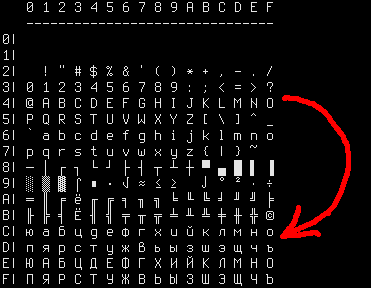
\includegraphics[width=0.5\textwidth]{fundamentals/koi8r.png}
\caption{KOI8-R table}
\end{figure}

Someone may notice that Cyrillic characters are allocated almost in the same sequence as Latin ones.
This leads to one important property: if all 8th bits in Cyrillic text encoded in KOI-8R are to be reset,
a text transforms into transliterated text with Latin characters in place of Cyrillic.
For example, Russian sentence:

\begin{framed}
\begin{quotation}
Мой дядя самых честных правил, Когда не в шутку занемог, Он уважать себя заставил, И лучше выдумать не мог.
\end{quotation}
\end{framed}

\dots if encoded in KOI-8R and then 8th bit stripped, transforms into:

\begin{framed}
\begin{quotation}
mOJ DQDQ SAMYH \^{}ESTNYH PRAWIL, kOGDA NE W [UTKU ZANEMOG, oN UWAVATX SEBQ ZASTAWIL, i LU\^{}[E WYDUMATX NE MOG.
\end{quotation}
\end{framed}

\dots perhaps this is not very appealing \ae{}sthetically, but this text is still readable to Russian language natives.

Hence, Cyrillic text encoded in KOI-8R, passed through an old 7-bit service will survive into transliterated, but still
readable text.

Stripping 8th bit is automatically transposes any character from the second half of
the (any) 8-bit \ac{ASCII} table to the first one, into the same place (take a look at red arrow right of table).
If the character has already been placed in the first half (i.e., it has been in standard 7-bit \ac{ASCII} table), it's not transposed.

Perhaps, transliterated text is still recoverable, if you'll add 8th bit to the characters which were seems
transliterated.

Drawback is obvious: Cyrillic characters allocated in KOI-8R table are not in the same sequence as
in Russian/Bulgarian/Ukrainian/etc. alphabet, and this isn't suitable for sorting, for example.

